%
% This is a borrowed LaTeX template file for lecture notes for CS267,
% Applications of Parallel Computing, UCBerkeley EECS Department.
%

\documentclass{article}
\usepackage{titlesec}
%\setlength{\oddsidemargin}{0.25 in}
%\setlength{\evensidemargin}{-0.25 in}
\setlength{\oddsidemargin}{0 in}
\setlength{\evensidemargin}{0 in}
\setlength{\topmargin}{-0.6 in}
\setlength{\textwidth}{6.5 in}
\setlength{\textheight}{8.5 in}
\setlength{\headsep}{0.75 in}
\setlength{\parindent}{0 in}
\setlength{\parskip}{0.1 in}


%
% ADD PACKAGES here:
%

\usepackage{amssymb}	% Already loads amsfonts
\usepackage{amsthm}
\usepackage{graphicx}
\usepackage{mathtools}	% Already loads amsmath
\usepackage{hyperref}
\usepackage{enumitem}
\usepackage{clrscode3e}  % for typesetting pseudocode
\usepackage{ulem}
\usepackage[usenames,dvipsnames]{xcolor}
\usepackage{multicol}


% Tikz and setup
\usepackage{tikz}
\usepackage{tikz-cd}
\usetikzlibrary{intersections, angles, quotes, calc, positioning}
\usetikzlibrary{arrows.meta}
\usepackage{pgfplots}
\pgfplotsset{compat=1.13}


\tikzset{
    force/.style={thick, {Circle[length=2pt]}-stealth, shorten <=-1pt}
}

%
% The following commands set up the lecnum (lecture number)
% counter and make various numbering schemes work relative
% to the lecture number.
%
\newcounter{lecnum}
\renewcommand{\thepage}{\thelecnum-\arabic{page}}
\renewcommand{\thesection}{\thelecnum.\arabic{section}}
\renewcommand{\theequation}{\thelecnum.\arabic{equation}}
\renewcommand{\thefigure}{\thelecnum.\arabic{figure}}
\renewcommand{\thetable}{\thelecnum.\arabic{table}}

%
% The following macro is used to generate the header.
%
\newcommand{\lecture}[5]{
   \pagestyle{myheadings}
   \thispagestyle{plain}
   \newpage
   \setcounter{lecnum}{#2}
   \setcounter{page}{1}
   \noindent
   \begin{center}
   \framebox{
      \vbox{\vspace{2mm}
    \hbox to 6.28in { {\bf #1
	\hfill} }
       \vspace{4mm}
       \hbox to 6.28in { {\Large \hfill Lecture #2: #3  \hfill} }
       \vspace{2mm}
       \hbox to 6.28in { {\it Lecturer: #4 \hfill Scribe: #5} }
      \vspace{2mm}}
   }
   \end{center}
   \markboth{Lecture #2: #3}{Lecture #2: #3}
   \vspace*{4mm}
}
\renewcommand{\cite}[1]{[#1]}
\def\beginrefs{\begin{list}%
        {[\arabic{equation}]}{\usecounter{equation}
         \setlength{\leftmargin}{2.0truecm}\setlength{\labelsep}{0.4truecm}%
         \setlength{\labelwidth}{1.6truecm}}}
\def\endrefs{\end{list}}
\def\bibentry#1{\item[\hbox{[#1]}]}

\newcommand{\fig}[3]{
			\vspace{#2}
			\begin{center}
			Figure \thelecnum.#1:~#3
			\end{center}
	}

% Colored theorem styles
\makeatother
\usepackage{thmtools}
\usepackage[framemethod=TikZ]{mdframed}
\mdfsetup{skipabove=1em,skipbelow=1em}

\declaretheoremstyle[
    headfont=\bfseries\sffamily\color{ForestGreen!70!black}, bodyfont=\normalfont,
    mdframed={
        linewidth=2pt,
        rightline=false, topline=false, bottomline=false,
        linecolor=ForestGreen, backgroundcolor=ForestGreen!5,
    },
    spaceabove=8pt
]{thmgreenbox}

\declaretheoremstyle[
    headfont=\bfseries\sffamily\color{NavyBlue!70!black}, bodyfont=\normalfont,
    mdframed={
        linewidth=2pt,
        rightline=false, topline=false, bottomline=false,
        linecolor=NavyBlue, backgroundcolor=NavyBlue!5,
    },
    spaceabove=8pt
]{thmbluebox}

\declaretheoremstyle[
    headfont=\bfseries\sffamily\color{NavyBlue!70!black}, bodyfont=\normalfont,
    mdframed={
        linewidth=2pt,
        rightline=false, topline=false, bottomline=false,
        linecolor=NavyBlue
    },
    spaceabove=8pt
]{thmblueline}

\declaretheoremstyle[
    headfont=\bfseries\sffamily\color{RawSienna!70!black}, bodyfont=\normalfont,
    mdframed={
        linewidth=2pt,
        rightline=false, topline=false, bottomline=false,
        linecolor=RawSienna, backgroundcolor=RawSienna!5,
    },
    spaceabove=8pt
]{thmredbox}

\declaretheoremstyle[
    headfont=\bfseries\sffamily\color{RawSienna!70!black}, bodyfont=\normalfont,
    numbered=no,
    mdframed={
        linewidth=2pt,
        rightline=false, topline=false, bottomline=false,
        linecolor=RawSienna, backgroundcolor=RawSienna!1,
    },
    qed=\qedsymbol,
    spaceabove=8pt
]{thmproofbox}

\declaretheoremstyle[
    headfont=\bfseries\sffamily\color{NavyBlue!70!black}, bodyfont=\normalfont,
    numbered=no,
    mdframed={
        linewidth=2pt,
        rightline=false, topline=false, bottomline=false,
        linecolor=NavyBlue, backgroundcolor=NavyBlue!1,
    },
    spaceabove=8pt
]{thmexplanationbox}

% Use these for theorems, lemmas, proofs, etc.
\theoremstyle{definition}
\declaretheorem[style=thmgreenbox, name=Definition, numberwithin=lecnum]{definition}
\declaretheorem[style=thmbluebox, numbered=no, name=Example]{example}
\declaretheorem[style=thmredbox, name=Theorem, numberwithin=lecnum]{theorem}
\declaretheorem[style=thmredbox, name=Proposition, sibling=theorem]{proposition}
\declaretheorem[style=thmredbox, name=Lemma, sibling=theorem]{lemma}
\declaretheorem[style=thmredbox, name=Corollary, sibling=theorem]{corollary}
% \newtheorem{theorem}{Theorem}[lecnum]
% \newtheorem{lemma}[theorem]{Lemma}
% \newtheorem{claim}[theorem]{Claim}
% \newtheorem{corollary}[theorem]{Corollary}
% \newtheorem{definition}[theorem]{Definition}
\declaretheorem[style=thmblueline, numbered=no, name=Remark]{remark}
\renewenvironment{proof}{{\bf \textit{Proof.}}}{\hfill\rule{2mm}{2mm}}
\makeatletter


% **** IF YOU WANT TO DEFINE ADDITIONAL MACROS FOR YOURSELF, PUT THEM HERE:

\renewcommand\Pr{\mathbb{P}}
\newcommand\Ex{\mathbb{E}}

\newcommand\N{\mathbb{N}}
\newcommand\Z{\mathbb{Z}}
\newcommand\Q{\mathbb{Q}}
\newcommand\R{\mathbb{R}}
\newcommand\C{\mathbb{C}}
\newcommand\F{\mathbb{F}}

\DeclarePairedDelimiter\ceil{\lceil}{\rceil}
\DeclarePairedDelimiter\floor{\lfloor}{\rfloor}
\DeclarePairedDelimiter\anglebrac{\langle}{\rangle}

\begin{document}
\lecture{MAT344 Intro to Combinatorics}{8}{Intro to Graph Theory}{Keegan Dasilva Barbosa}{Kevin Gao}

\section{Eulerian Graphs and Circuit}

\begin{definition}[Eulerian Circuit]
    Given a graph $G = (V,E)$, an \textit{\textbf{Eulerian circuit}} is a sequence of vertices $x_0,\ldots,x_t$ such that
    \begin{itemize}
        \item $x_0 = x_t$ 
        \item $\forall i \in [t].\, \{x_i, x_{i+1}\} \in E$ 
        \item $\forall e \in E.\, \exists \text{ unique $i \in [t]$.}\, e = \{x_i, x_{i+1}\}$ (i.e. every edge appears exactly once in an Eulerian circuit)
    \end{itemize}
\end{definition}

We say a graph is \textit{\textbf{Eulerian}} if and only if it has an \textbf{Eulerian circuit}. An Eulerian circuit is also referred to as an \textbf{Euler tour} in some texts. The notion of an Eulerian circuit and graph appears in the famous problem of the \textbf{bridges of K\"onigsberg}.

In 1736, Euler gave his famous characterization of an Eulerian graph, stated as follows

\begin{theorem}[Euler, 1736]
    A connected graph $G = (V,E)$ is Eulerian if and only if all its vertices have even degree.
\end{theorem}

\begin{proof}
    The forward direction of the proof is quite straightforward whereas the reverse direction requires a slightly more involved proof by induction.

    ($\implies$): Let $G$ be a connected graph. Assume that $G$ is Eulerian so it must have an Eulerian circuit. Note that in an Eulerian circuit, every time we enter a vertex, we must also leave the vertex. This is the case for all vertices because otherwise we would have an infinite graph. Hence, all vertices in $G$ must have even degree.

    $(\impliedby)$: Let $G$ be a graph. We proceed by strong induction on the number of edges.

    \textbf{Base Case}: $G$ is a graph with $m = 0$ edge. The result trivially holds.

    \textbf{Inductive Step}: Let $m \in \N$ be arbitrary. Assume that for all $k \in \N$ such that $0 \leq k < m$, the implication holds. Let $G = (V,E)$ be a connected graph with $m$ edges. Further, assume that $\deg_G(v)$ is even for all $v \in V$. Since the graph is connected and every vertex has even degree, it follows immediately that $\deg_G(v) \geq 2$ for all $v \in V$. This also implies that $G$ contains a cycle. Let $c = v_1\ldots v_k$ be such cycle of maximal length and $E'$ be the edges contained in this cycle.

    If $c$ contains all edges exactly once, we are done. Hence, suppose $E' \neq E$ and consider the graph $G' = (V, E \setminus E')$. It has connected components $S_1, \ldots, S_l$. Since $E' \neq E$, each of the connected components $S_i$ contains strictly fewer edges than $|E| = m$. For every $v \in G$, an even number of edges of $G$ at $v$ are in the cycle $c$, so we we remove these edges, each vertex in the remaining graph should still have even degree. Apply the induction hypothesis to the components, which asserts that each of the components $S_1, \ldots, S_l$ possess an Eulerian circuit. Further, since $c$ is a cycle, $C = (\{v_1,\ldots,v_k\}, E')$ itself is also Eulerian. Now, we recursively construct an Eulerian circuit, say $x$, in the original graph $G$. Start from $v_1$, find the component $S_i$ containing $v_1$, and concatenate the Eulerian tour in $S_i$ to $x$. Next, move from $v_1$ to $v_2$ along $\{v_1,v_2\} \in E'$. If $\{v_1,v_2\} \not\in E$, then they must have been in the same connected component, in which case we skip $v_2$ and move to $v_3$. Repeat this until we have walked through every edge in each one of the $l$ connected components and the edges in $E'$ connecting each component. It is clear that $x$ is Eulerian since it visits every edge exactly once.

    By induction, the implication holds.
\end{proof}

\begin{figure}[htbp]
    \centering
    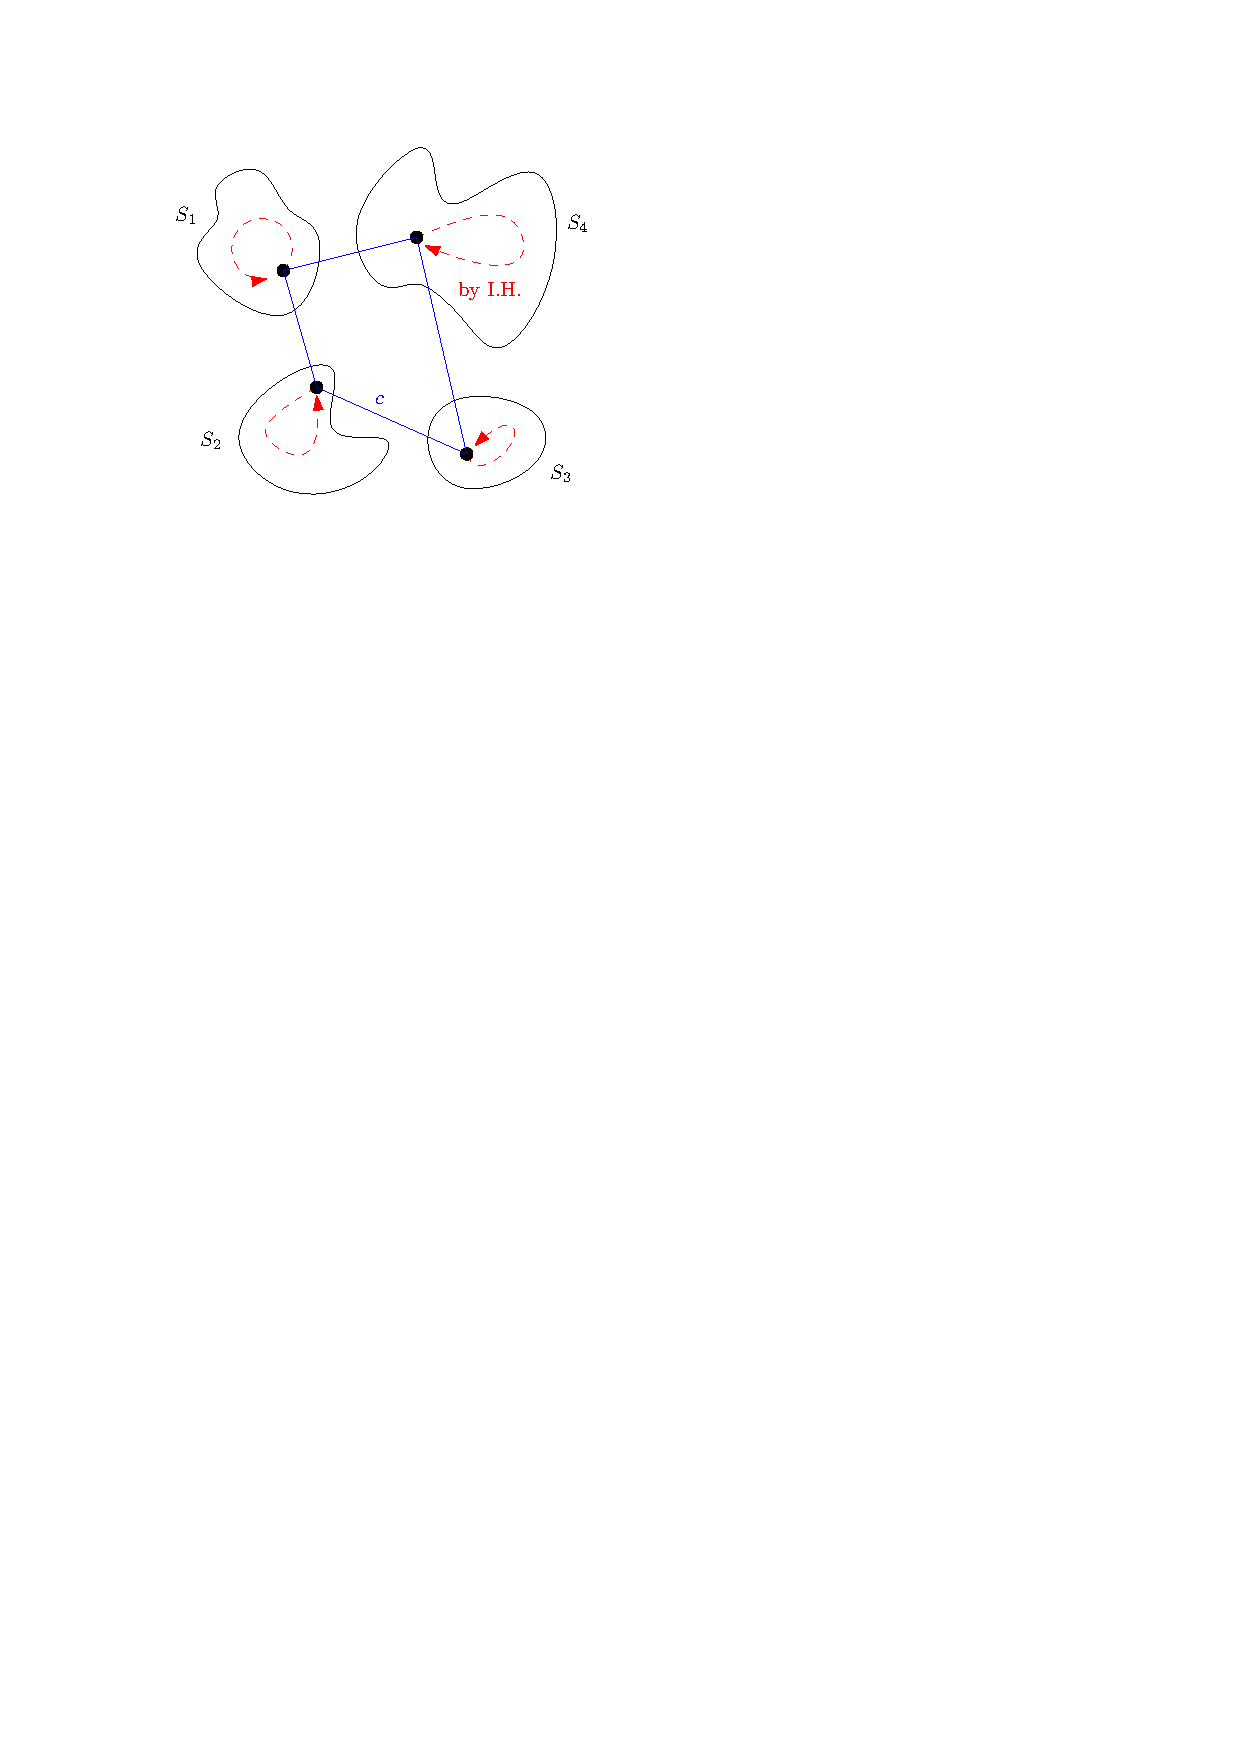
\includegraphics[width=0.3\linewidth]{figures/eulerian-circuit-construct.pdf}
    \caption{Construct an Eulerian circuit in the original graph $G$ by first finding a cycle $c$, remove the cycle, find an Eulerian circuit within each component $S_1,\ldots,S_l$, and concatenate these circuits via the cycle $c$.}
    \label{fig:euler-circuit-construct}
\end{figure}

\section{Hamiltonian Graphs}

\begin{definition}[Circuits]
    A \textit{\textbf{circuit}} in a graph $G = (V,E)$ is a sequence of distinct vertices $v_1,\ldots,v_k$ such that for all $i \in \{1,\ldots, k-1\}$, $\{v_i,v_{i+1}\} \in E$ and $\{v_k,v_1\} \in E$. Note, a circuit induces a copy of a subgraph isomorphic to $C_k$ for $k \geq 3$. Specially, we define a \textbf{single vertex} a circuit as well.
\end{definition}

\begin{definition}[Hamiltonian Graph]
    We call a graph with $n$ vertices \textit{\textbf{Hamiltonian}} if it admits a circuit of length $n$, which is to say that the graph has a spanning subgraph that is isomorphic to $C_n$.
\end{definition}

A sufficient condition for Hamiltonian graphs.

\begin{theorem}[Dirac, 1952]
    Let $G = (V,E)$ be a graph with $n$ vertices where $n \geq 3$. Suppose that for every $v \in V$, $\deg_G(v) \geq \ceil{\frac{n}{2}}$. Then, $G$ is Hamiltonian.
\end{theorem}

\begin{proof}
    Let $G = (V,E)$ be a graph with $n \geq 3$ vertices. Assume that $\deg_G(v) \geq \ceil{\frac{n}{2}}$ for all $v \in V$. Let $\delta(G)$ denote the minimum degree. That is, $\delta(G) = \min \{\deg_G(v) \mid v \in V\}$. Then, the assumption is equivalent to that $\delta(G) \geq \ceil{\frac{n}{2}}$.
    
    We claim that $G$ is connected. We prove the claim by contradiction. So suppose not, consider the component $G' = (V_{G'}, E_{G'})$ of $G$ with the fewest number of vertices. Since $\delta(G) \geq \ceil{\frac{n}{2}}$, each vertex is connected to at least $\ceil{\frac{n}{2}}$ other vertices. Since $C$ is a component that is not connected to vertices in other components, $|V_{G'}| \leq \ceil{\frac{n}{2}}$. But then, $\delta(G') < |V_C| \leq \ceil{\frac{n}{2}}$, which contradicts the assumption that $\deg_G(v) \geq \ceil{\frac{n}{2}}$ for all $v \in V$, including those in $G'$.

    Since $G$ is connected, we can find the longest path in $G$. Let $P = v_0 \ldots v_k$ be a longest path in $G$ of length $k$ (with $k$ edges and $k+1$ vertices). We claim that there exists some $0 \leq i \leq k-1$ such that $\{v_0,v_{i+1}\} \in E$, $\{v_i, v_k\} \in E$, and $\{v_i, v_{i+1}\} \in E$ as shown in Figure \ref{fig:dirac-thm-path}.

    \begin{figure}[htbp]
        \centering
        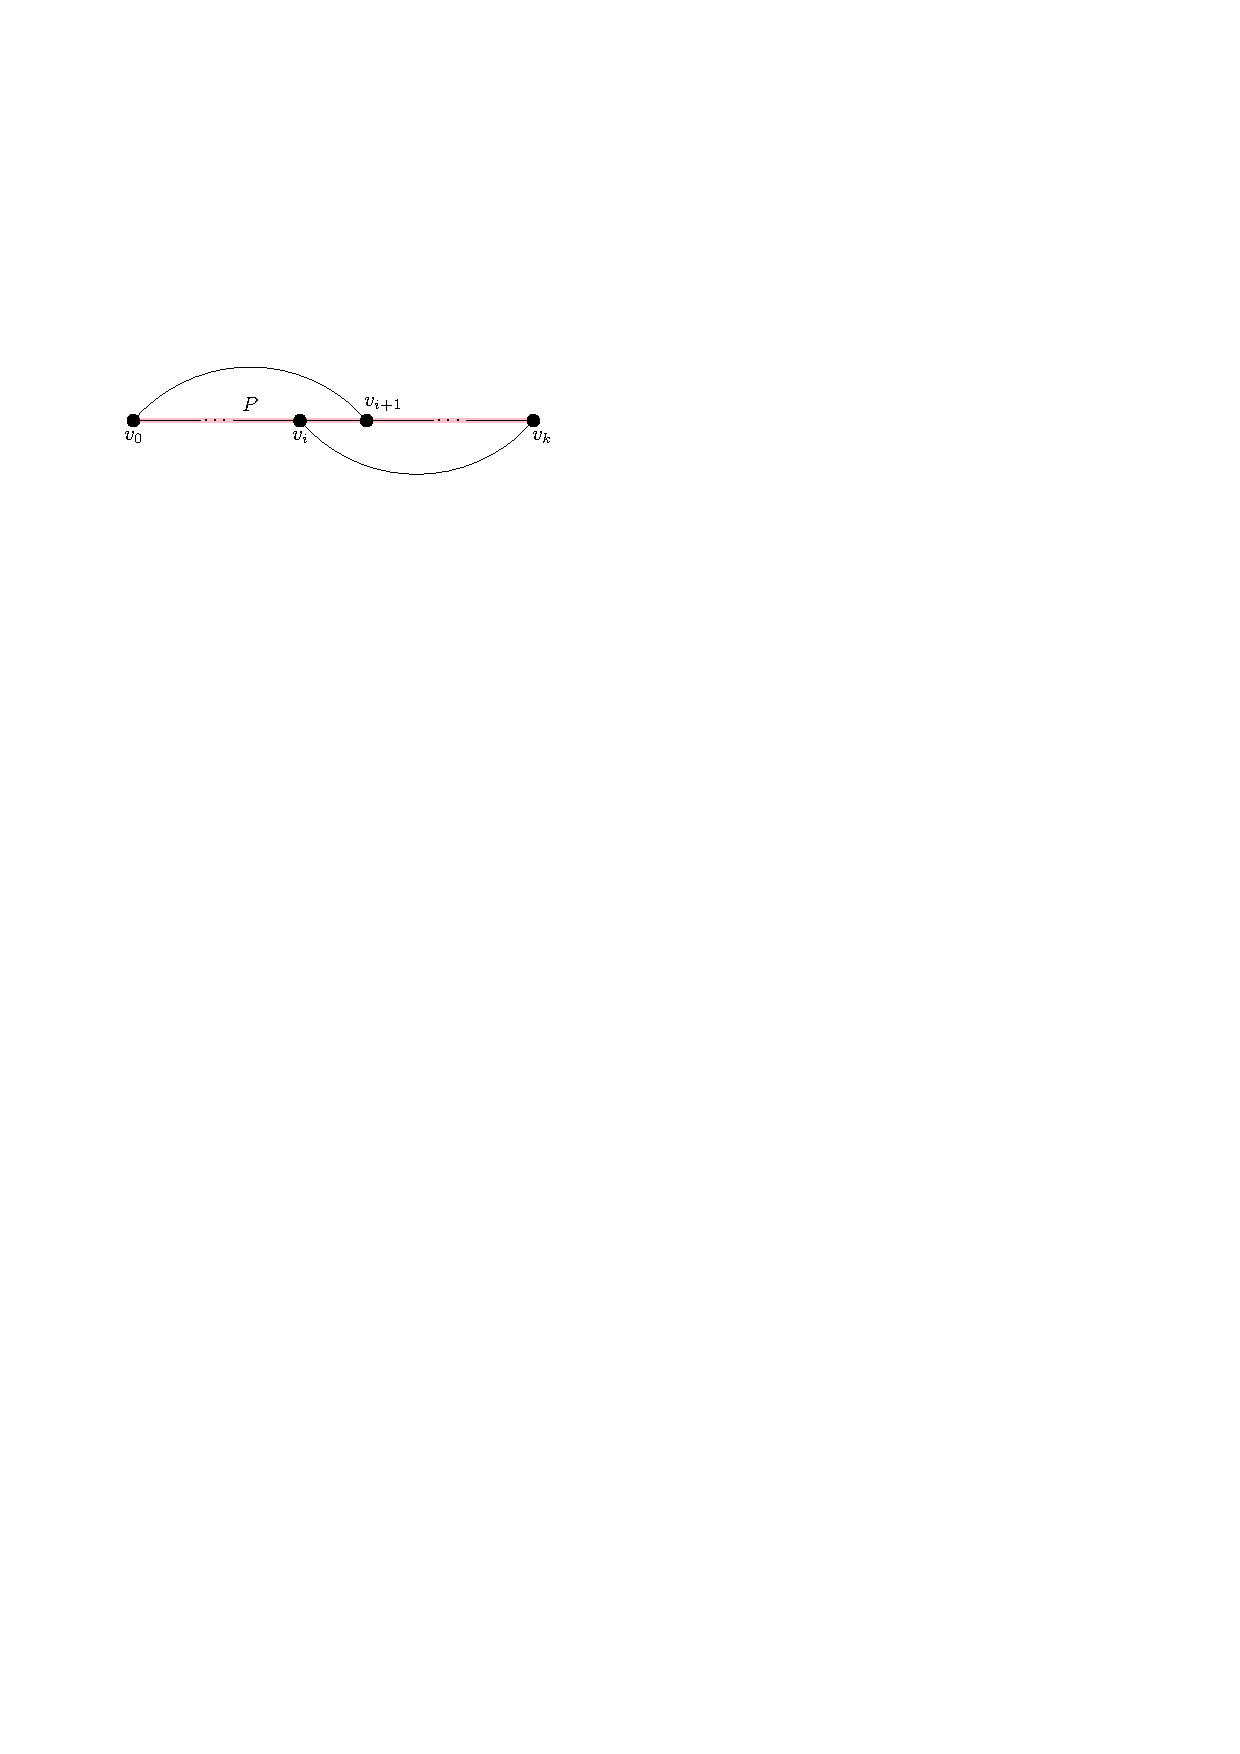
\includegraphics[width=0.4\linewidth]{figures/dirac-thm-path.pdf}
        \caption{The longest path $P = v_0\ldots v_k$ with $k+1$ vertices is colored in red. There exists some $0 \leq i \leq k$ such that $\{v_0,v_{i+1}\} \in E$ and $\{v_i,v_k\} \in E$.}
        \label{fig:dirac-thm-path}
    \end{figure}

    Such adjacent vertices $v_i$ and $v_{i+1}$ such that $v_i$ is adjacent to $v_k$ and $v_{i+1}$ is adjacent to $v_0$ must exists. By way of contradiction, suppose $v_i$ and $v_{i+1}$ do not exist. Then, for every vertex adjacent to $v_0$, there must exists some vertex adjacent to it that is NOT adjacent to $v_k$. Similarly, for every vertex adjacent to $v_k$, there must exists some adjacent vertex that is NOT adjacent to $v_0$. Note that these two sets of vertices are disjoint and do not include $v_k$. This implies that
    $$
    \deg_G(v_0) + \deg_G(v_k) + 1 \leq k + 1
    $$
    since we are not overcounting and the number of vertices being counted is at most the length of path $P$. The additional 1 on the LHS of the inequality came from couting $v_k$ as it is not included in either $\deg_G(v_0)$ or $\deg_G(v_k)$. Now, since $\deg_G(v) \leq \ceil{\frac{n}{2}}$ for all $v \in V$,
    $$
    n + 1 \leq \left\lceil \frac{n}{2} \right\rceil + \left\lceil \frac{n}{2} \right\rceil + 1 \leq \deg_G(v_0) + \deg_G(v_k) + 1 \leq k + 1
    $$
    so $n + 1 \leq k+1$. This implies that $n < k+1$ since both $n$ and $k$ are integers. But this leads to a contradiction because the number of vertices on the path $P$ cannot be more than the total number of vertices in the entire graph.

    The existence of such $v_i$ and $v_{i+1}$ allows us to construct a cycle $C = v_0 \to v_{i+1} \leadsto_{P} v_k \to v_i \leadsto_{P} v_0$. We claim this cycle is Hamiltonian.

    \begin{figure}[htbp]
        \centering
        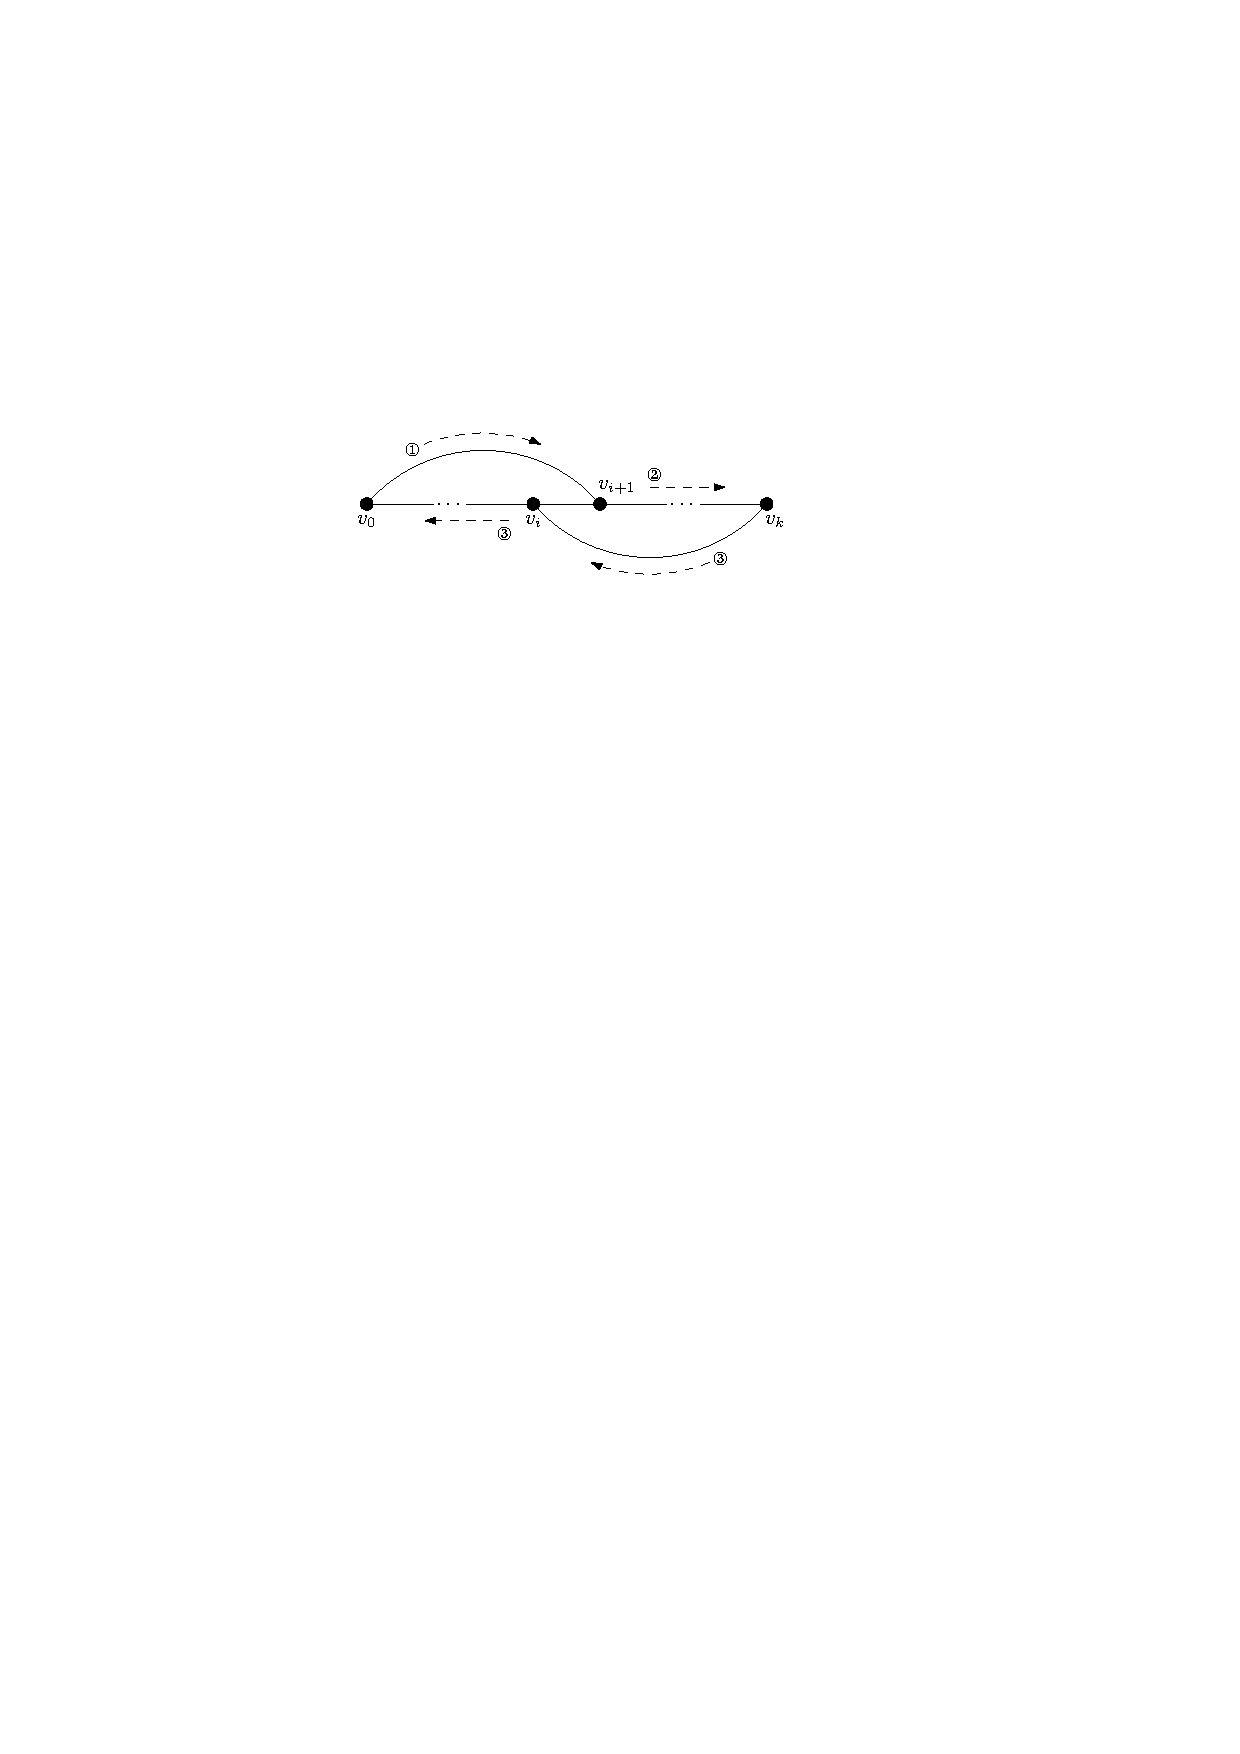
\includegraphics[width=0.4\linewidth]{figures/dirac-thm-hamcycle.pdf}
        \caption{The Hamiltonian path is $C = v_0 \to v_{i+1} \leadsto_{P} v_k \to v_i \leadsto_{P} v_0$.}
        \label{fig:dirac-thm-hamcycle}
    \end{figure}

    To see why $C$ is Hamiltonian, again we use a contradiction proof. Suppose $C$ is not Hamiltonian. Then, by definition, there must be some vertex $w \in V$ such that $w$ is not on $C$. But since $G$ is connected, $w$ must be adjacent to some vertices, say $v_w \in V$. Without loss of generality, suppose that this $v_w$ is on the cycle $C$. There must also be a $v_{w+1}$ immediately adjacent to $v_w$. By construction, the cycle $C$ contains $k+1$ edges (that's all edges on $P$ along with $\{v_0,v_{i+1}\}, \{v_i,v_k\}$ and without $\{v_i,v_{i+1}\}$). We then consider the path from $v_w$ to $v_{w+1}$ by following the edges on the cycle. This leads to a path of length $k$, namely $p = v_w \leadsto v_0 \to v_{i+1} \leadsto v_k \to v_i \leadsto v_{w+1}$. Now, we extend the left end of this path to $w$ since $w$ is adjacent to $v_w$ and still get back a valid path. The new path $P' = w \to v_w \leadsto v_0 \to v_{i+1} \leadsto v_k \to v_i \leadsto v_{w+1}$ is one edge longer than $p$. However, this contradicts the maximality assumption for $P$ since now we would have a path, $P'$, that contains more vertices than $P$. Therefore, $C$ is indeed a Hamiltonian path.

    \begin{figure}[htbp]
        \centering
        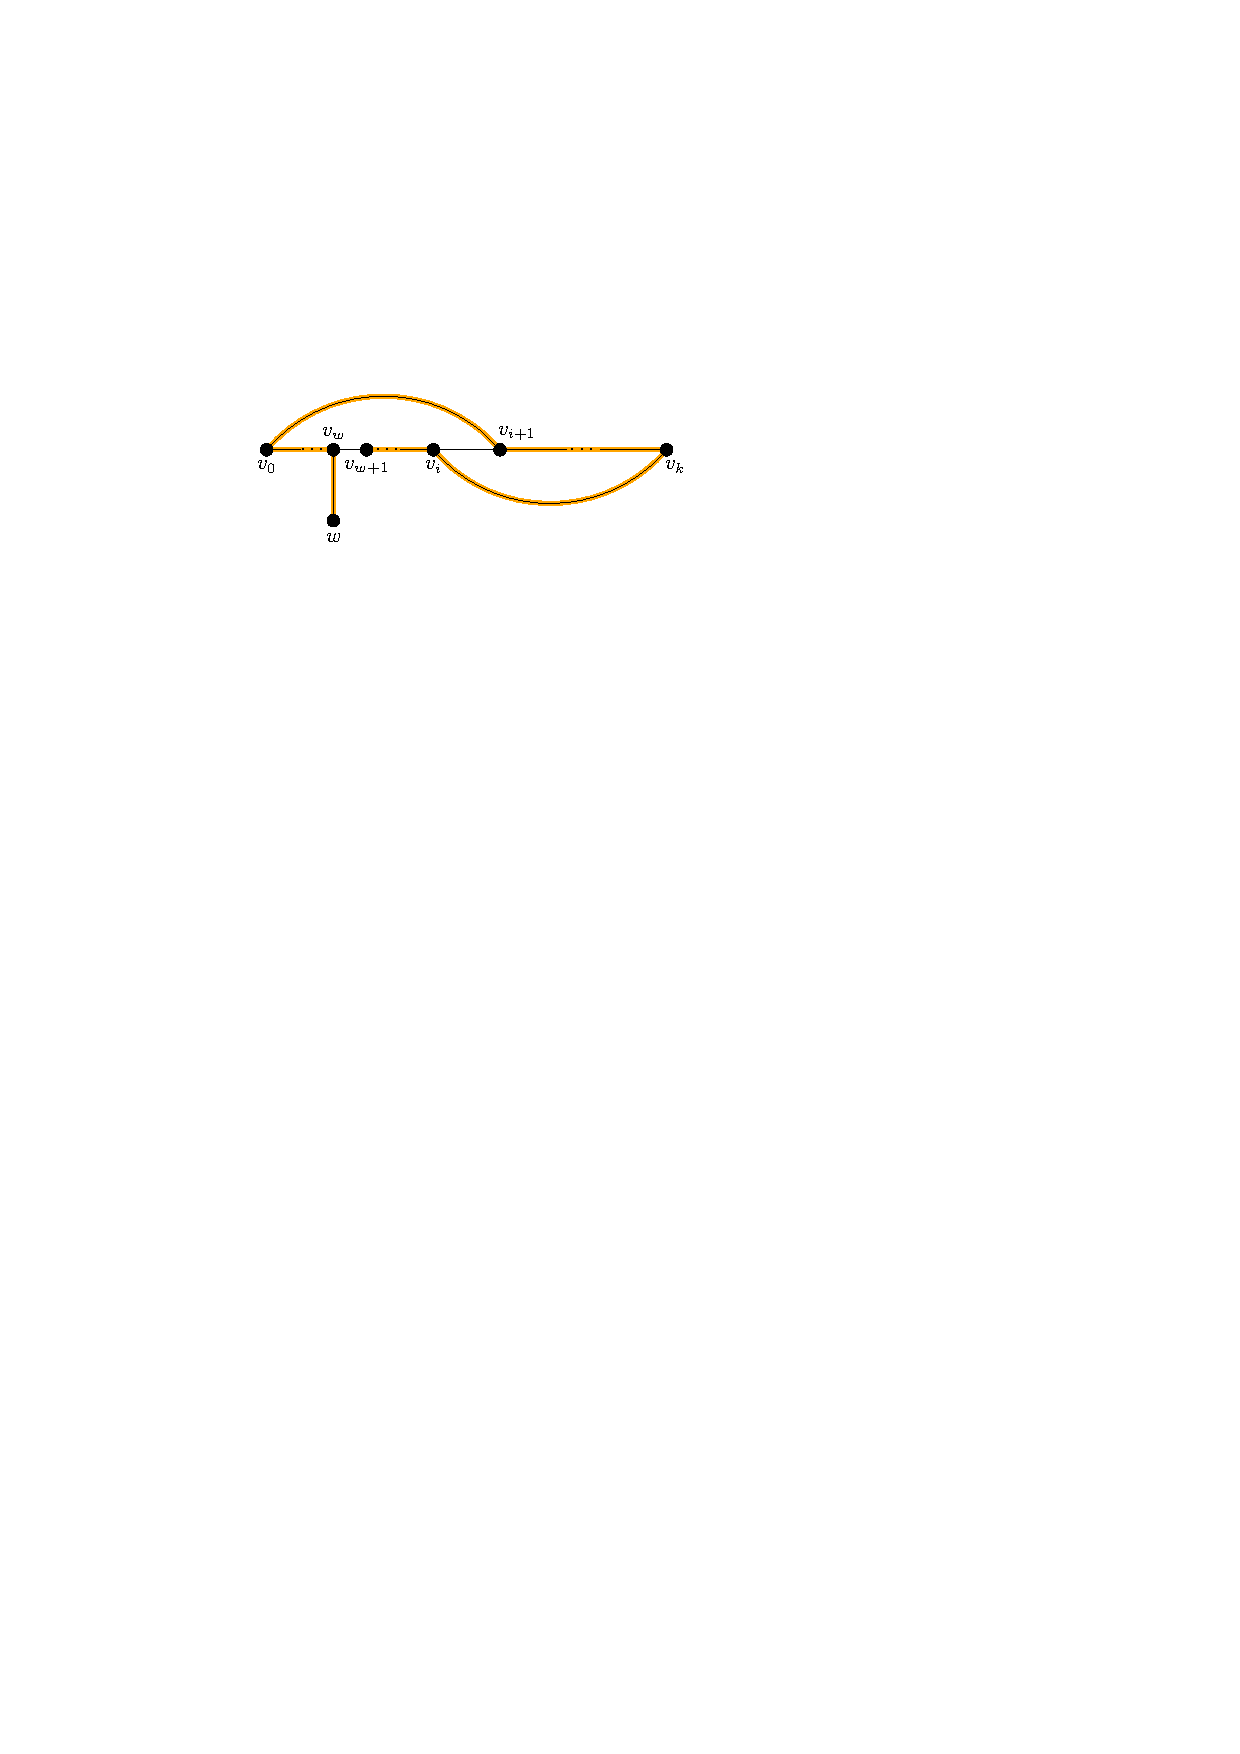
\includegraphics[width=0.4\linewidth]{figures/dirac-thm-longer-path-contradiction.pdf}
        \caption{With the existence of a vertex $w$ outside of the previously constructed cycle, we would have a longer path (colored in orange), contradicting the maximality of $P$.}
        \label{fig:dirac-thm-path-contradiction}
    \end{figure}

    It follows immediately that $G$ is Hamiltonian by definition.
\end{proof}

\section{Graph Coloring}

\subsection{Independent Sets and Bipartite Graphs}

\begin{definition}[Independent Set]
    Given a graph $G = (V,E)$, we say $A \subseteq V$ is \textit{\textbf{independent}} if and only if no no vertices in $A$ are adjacent.
\end{definition}

The only independent sets in $K_n$ are singletons. We can prove this using a contradiction and the definition of a complete graph and independent set.

\begin{definition}[Bipartite Graph]
    We say a graph $G = (V,E)$ is \textit{\textbf{bipartite}} if and only if we can partition $V$ into two \textbf{disjoint} \textbf{independent} sets.
\end{definition}

A bipartite graph $(V_1 \cup V_2, E)$ is a complete bipartite graph iff every $v_1 \in V_1$ is connected to every vertex in $V_2$ and vice versa. We denote a complete bipartite graph by $K_{|V_1|,|V_2|}$ ($K$ with a subscript denoting the size of the left and right partition, respectively).

\begin{theorem} \label{thm:odd-length-cycle-bipartite}
    A graph is bipartite if and only it does not contain a circuit of odd length.
\end{theorem}

\begin{proof}
    \hfill

    ($\implies$): Let $G=(V,E)$ be a bipartite graph. In particular, $V = A \cup B$ for some $A,B \subseteq V$ such that $A \cap B = \emptyset$ and for all $\{a,b\} \in E$, $a \in A$ and $b \in B$. Suppose, for contradiction, that $G$ contains an odd-length cycle $C = v_1 v_2 \ldots v_{n} v_1$ of length $n$. Without loss of generality, suppose that $v_i$ and $v_{i+1}$ alternates between $A$ and $B$. So, $v_1 \in A$, $v_2 \in B$, $v_3 \in A$, and so on. If the cycle is not in that particular order, we can reindex the vertices and still have the same cycle.

    Then, for $k \in \{1,2,3,\ldots,n\}$,
    $$
    v_k \in \begin{cases}
        A & \text{$k$ is odd} \\
        B & \text{$k$ is even}
    \end{cases}
    $$
    Since $C$ is a cycle of odd length, $n$ is odd. It follows that $v_n \in A$. But then, since $v_1 \in A$ and $\{v_n, v_1\} \in E$, this is a contradiction to the assumption that $G$ is bipartite.

    ($\impliedby$): Let $G=(V,E)$ be a graph. Without loss of generality, assume that $G$ is connected. Otherwise, we can consider the connected components individually. Assume that $G$ contains no odd cycle. Let $w \in V$ be a vertex in $G$.

    Let $A$ be the set of vertices whose shortest distance from $w$ is even, and let $B$ be the set of vertices whose shortest distance from $w$ is odd. That is,
    $$
    \begin{aligned}
        A = \{ v \in V \mid d(v,w) \equiv 0 \mod 2 \} \\
        B = \{ v \in V \mid d(v,w) \equiv 1 \mod 2 \}
    \end{aligned}
    $$
    Since $G$ is connected, every vertex is either at an even distance or odd distance from $w \in V$. A vertex cannot be both at an even distance and an odd distance from $w$ at the same time. Hence, $A \cup B = V$ and $A \cap B = \emptyset$. This implies that $A$ and $B$ are a valid partition of $V$.
    
    Now, we would like to show that $G$ is bipartite. It suffices to show for all vertices $a_1,a_2 \in V$ and $b_1,b_2 \in B$, $\{a_1,a_2\} \not\in E$ and $\{b_1,b_2\} \not\in E$. To prove this fact, we suppose the contrary and derive a contradiction. So, suppose that there does exist such $x,y \in A$ or $x,y \in B$ such that $\{x,y\} \in E$. Fix such $x,y$. We can assume that $x \neq y \neq w$. Otherwise, we have $w = x$ and $d(x,w) = 0$. Since $x$ and $y$ are in the same partition, $d(y,w)$ is even and $d(y,x) = 0$. However, this is not possible since $d(y,x) = 1$, which is odd. By a similar argument, we can show that $w \neq y$ either.
    
    To obtain a contradiction, we consider the shortest path from $x$ to $w$ and the shortest path from $y$ to $w$. Let $p$ be the shortest path from $x$ to $w$, and let $q$ be the shortest path from $y$ to $w$. Let $z$ be the last common vertex of $p$ and $q$. Note that $z$ may be $w$. We also note that $|p|$ and $|q|$ have the same parity since we assumed that $y,x$ are in the same partition.

    \begin{figure}[htbp]
        \centering
        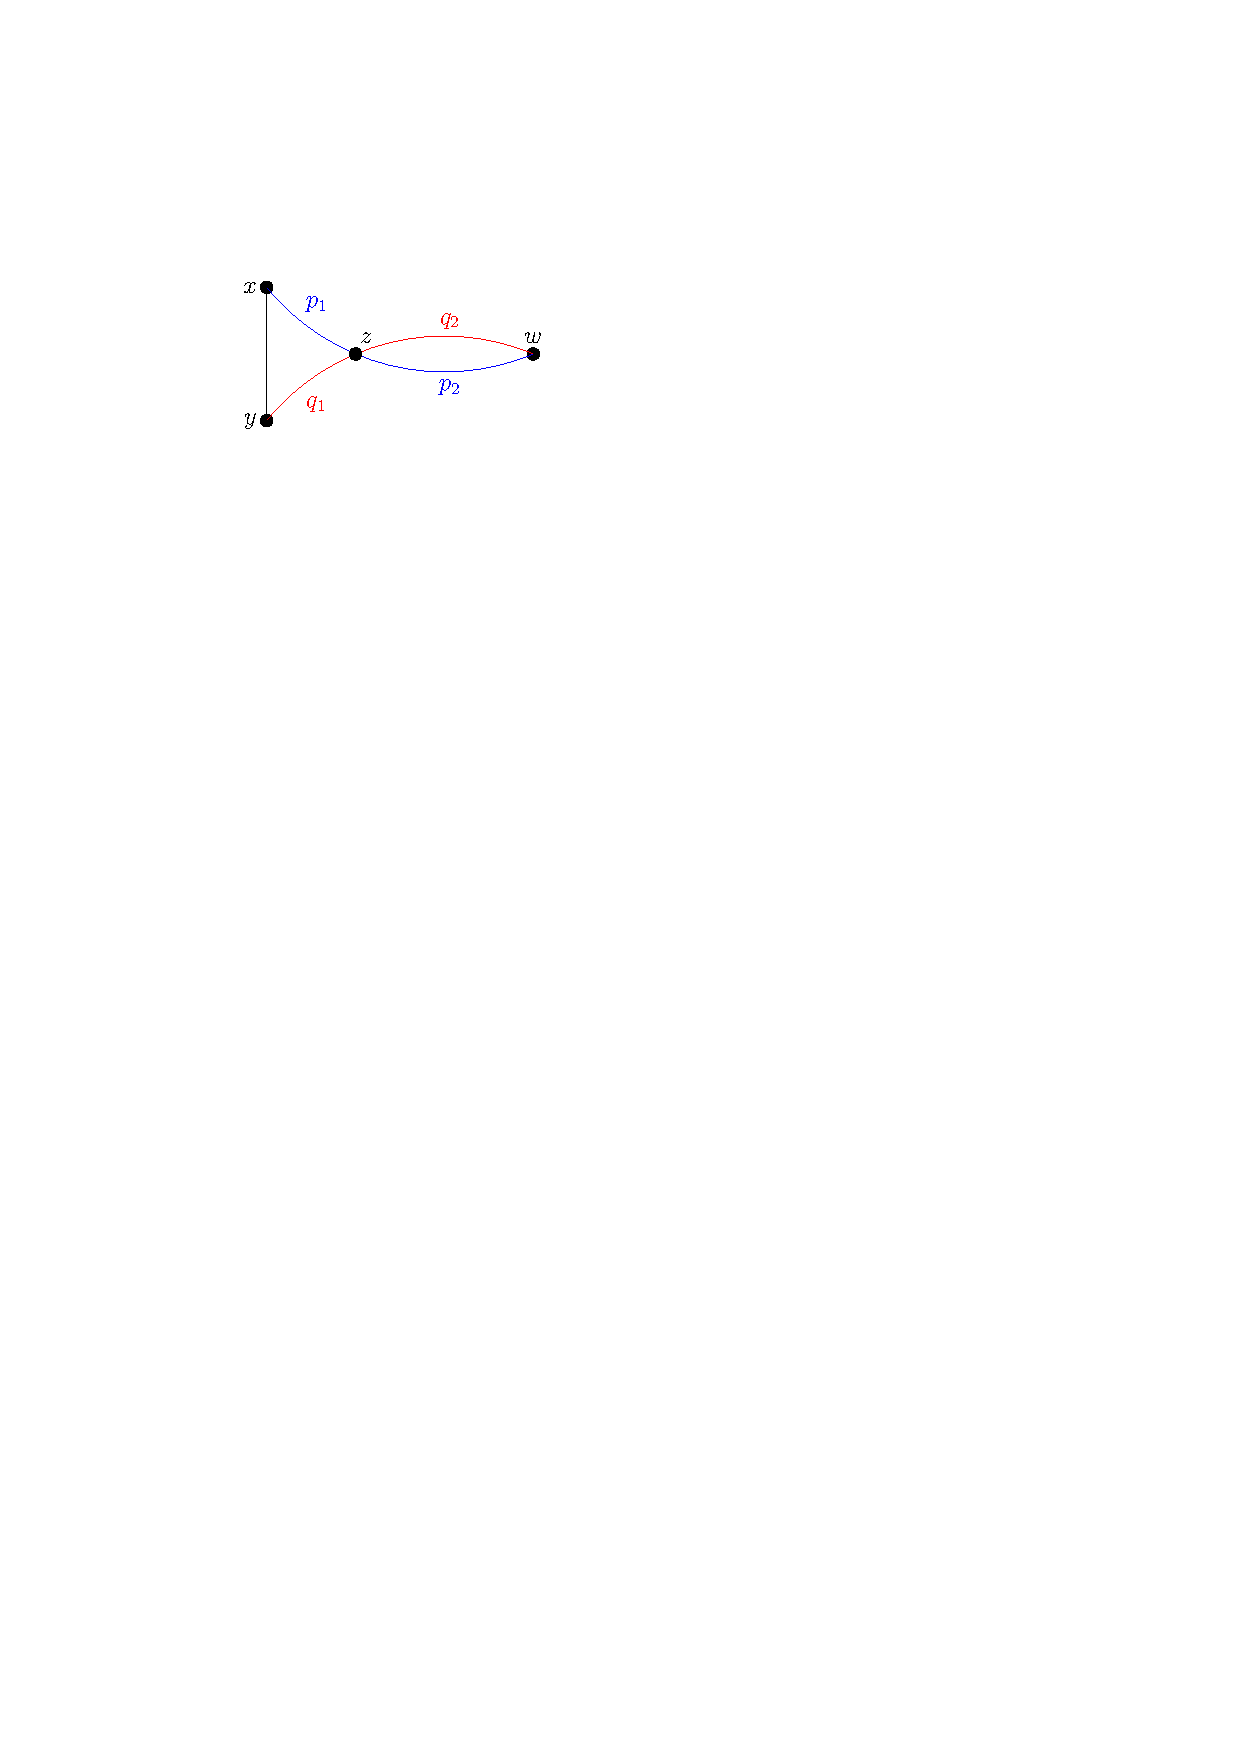
\includegraphics[width=0.3\linewidth]{figures/odd-length-cycle-bipartite.pdf}
        \caption{$p$ is the shortest path from $x$ to $w$. $q$ is the shortest path from $y$ to $w$. $p_1$ is the part of $p$ from $x$ to the last common vertex of $p$ and $q$. Similarly, $q_1$ is the part of $q$ from $y$ to the last common vertex of $p$ and $q$.}
        \label{fig:odd-length-cycle-bipartite}
    \end{figure}
    
    Let $p_1 = x \leadsto_p z$ be the part of the path $p$ from $x$ to $z$. Similarly, let $p_2 = z \leadsto_p w$, $q_1 = y \leadsto_q z$, and $q_2 = z \leadsto_q w$. We claim that $|p_2| = |q_2|$ since otherwise we can obtain a shorter path from $x$ to $w$ or from $y$ to $w$. Further, we claim that $|p_1|$ and $|q_1|$ have the same parity becuase $|p|$ and $|q|$ have the same parity and the second part of both paths, $p_2$ and $q_2$, are of the same length. Recall that $\{x,y\} \in E$. Then, $C = x \leadsto_{p_1} z \leadsto_{q_1} y \to x$. Since $|p_1|$ and $|q_1|$ have the parity, $|C| = |p_1| + |q_1| + 1$ is odd. This is becuase $|p_1| + |q_1|$ can be expressed as $2k$ for some $k \in \Z$. This is an odd-length cycle, which is a contradiction to our initial assumption that $G$ has no odd cycle. The only additional assumption leading to this contradiction is that $G$ is not bipartite. Hence, $G$ must be bipartite.
\end{proof}

\subsection{Coloring}

\begin{definition}[Proper Coloring]
    Let $G = (V,E)$ be a graph. A (proper) \textit{\textbf{coloring}} of $G$ is a function $\phi:\; V \to [k]$ such that for all $i \in [k]$, $\phi^{-1}(i)$ is independent. Equivalently, $\phi$ is a (proper) coloring of $G$ iff $\forall \{a,b\} \in E.\, \phi(a) \neq \phi(b)$. We call $\phi$ a $k$-coloring.
\end{definition}

\begin{definition}[Chromatic Number]
    The \textit{\textbf{chromatic number}} of a graph $G$, is the smallest $k$ such that there is a proper $k$ coloring of $G$. The chromatic number of $G$ is denoted by $\chi(G)$.
\end{definition}

\begin{theorem}
    A graph is 2-colorable if and only if it does not contain an odd-length cycle.
\end{theorem}

\begin{proof}
    Theorem \ref{thm:odd-length-cycle-bipartite} states that a graph is bipartite iff there is no odd-length cycle. To prove this theorem, it suffices to prove that a graph is 2-colorable if and only if the graph is bipartite.

    ($\implies$): Let $G = (V,E)$ be a 2-colorable graph. Take the coloring. Assign vertices with one color to $V_1$ and vertices with another color to $V_2$. $V_1$ and $V_2$ is a partition of $V$. By definition of a 2-color, for all $x,y \in V_1$, $\{x,y\} \not\in E$ and for all $x,y \in V_2$, $\{x,y\} \not\in E$.

    ($\impliedby$): Let $G=(V,E)$ be a bipartite graph where $V = V_1 \cup V_2$ is a partition. Assign one color to all vertices in $V_1$ and assign another color to all vertices in $V_2$. It is easy to prove that this is a valid 2-coloring directly from the definition of a bipartite graph.
\end{proof}

To demonstrate the concept of graph coloring and chromatic number, we consider the Petersen graph.

\begin{figure}[htbp]
    \centering
    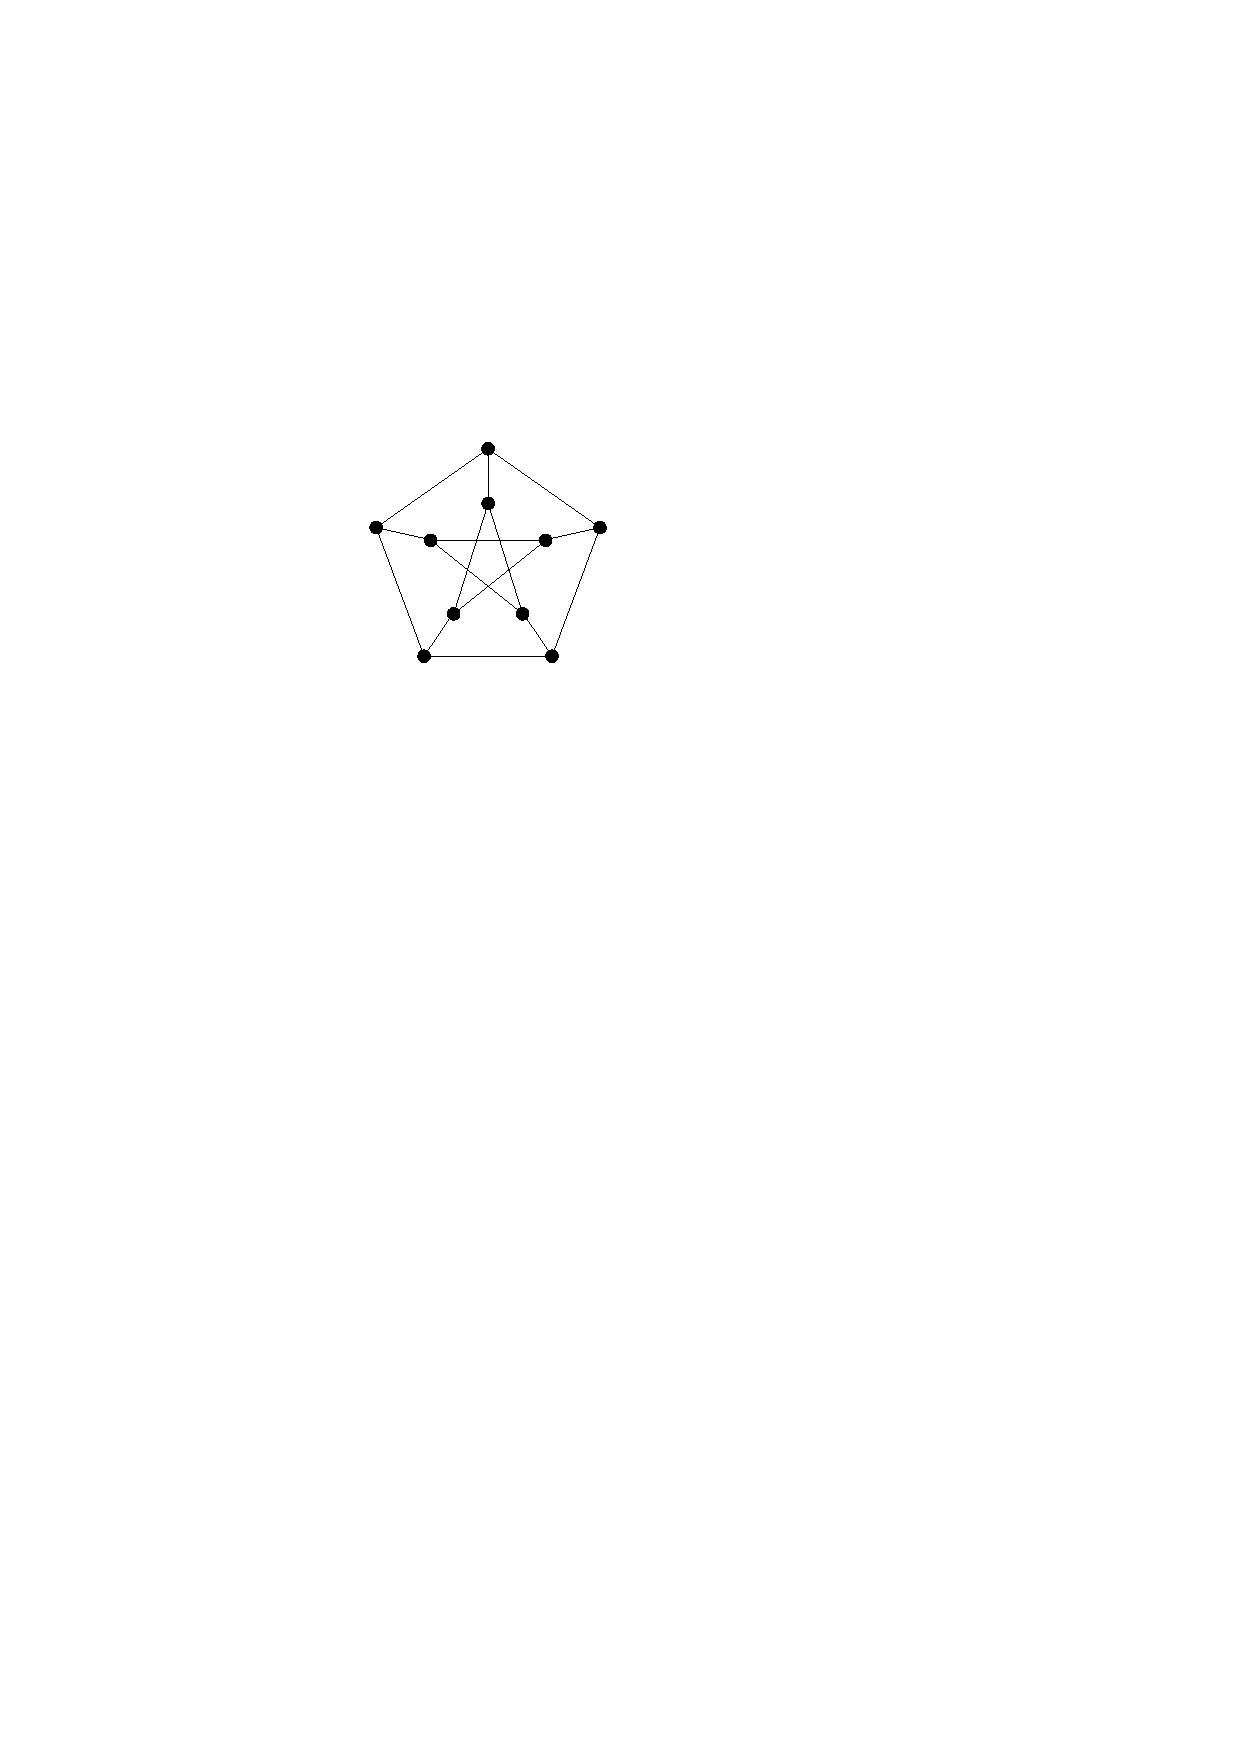
\includegraphics[width=0.2\linewidth]{figures/peterson-graph.pdf}
    \caption{The Petersen graph.}
    \label{fig:petersen-graph}
\end{figure}

\end{document}